\documentclass[../main]{subfiles}
\begin{document}

\section{
  Brainfuck parsing and code generation
}

Now that we introduced the various techniques to generate programs from
pointer trees generated by \gls{constexpr} functions, we will use them in the
context of compile-time parsing and code generation for the Brainfuck language.
Therefore use data structures and code generation techniques introduced in
subsection \ref{lbl:ptr-tree-codegen}.

\subsection{
  Constexpr Brainfuck parser and AST
}

\subsubsection{
  AST
}

The Brainfuck AST is defined in the header shown in appendix \ref{app:bf-ast}.
The header file also contains helper function definitions to handle AST nodes
safely, such as \lstinline{visit} which will be used in one of the
code generation backends.

Here are the main data types:

\begin{itemize}
\item
\lstinline{node_interface_t}, which is a common base type for all AST nodes.

\item
\lstinline{ast_token_t}, which represents a single AST token.

\item
\lstinline{ast_block_t}, which represents an AST block, which simply is a
\lstinline{std::vector} of \lstinline{std::unique_ptr<node_interface_t>}.

\item
\lstinline{ast_while_t}, which represents a while conditional block.
The instruction block itself is contained in an \lstinline{ast_block_t} value.

\end{itemize}

The implementation of the AST are available in appendix \ref{app:bf-ast}
where you can observe that all the types are implemented as they would be
for a regular Brainfuck parser, except all their methods are \gls{constexpr}.

\begin{lstlisting}[
  language=c++,
  caption=Definition of the AST visitor function,
  label=lst:bf-ast-visit-def
]{}
template <typename F>
constexpr auto visit(F f, ast_node_ptr_t const &p) {
  switch (p->get_kind()) {
  case ast_token_v:
    return f(static_cast<ast_token_t const &>(*p));
  case ast_block_v:
    return f(static_cast<ast_block_t const &>(*p));
  case ast_while_v:
    return f(static_cast<ast_while_t const &>(*p));
  }
}
\end{lstlisting}

The \lstinline{visit} function implementation also looks like a regular \cpp
function as shown in listing \ref{lst:bf-ast-visit-def}.
It is a higher order function that allows recursive operations on the AST to be
carried in a type-safe manner.

\subsubsection{
  Parser
}

The Brainfuck parser, again, looks like nothing special. For that reason I will
not get into the implementation details. The function definition is available
in appendix \ref{app:bf-parser}.

On the surface: the parser takes a pair of begin and end iterators as an input.
It parses Brainfuck tokens until it reaches the end iterator or a while end
token, and returns a pair containing an iteretor pointing after the last parsed
token and the parsing result.

When a while begin token is reached, it calls itself recursively and resumes
parsing at the position of the iterator returned by the callee, which is right
after the while block.

The main parsing function implementation (including the function prototype)
is very condensed: it fits in 40 lines of code with a max line width set to 84.
It is no different from a regular Brainfuck parsing function except for it being
\gls{constexpr}, and it can actually be used as a regular \cpp program.

These make it much easier to debug as it can be ran through a \cpp debugger like
GDB or LLDB, and also more maintainable as it does not require any
template metaprogramming experience to understand the implementation.
Additionally, \gls{constexpr} execution enforces checks on memory allocations and
deallocations as well as memory bound checking. Therefore testing functions
in \gls{constexpr} contexts can help finding memory safety issues.

\subsection{
  A variety of techniques to generate code from a dynamic AST
}

Once the \gls{constexpr} parser is implemented, the next step consists in
figuring out how to transform its result, which contains dynamic memory,
into \cpp code.

As you may remember from subsection \ref{lbl:constexpr-programming},
there is no direct way to use values holding pointers to dynamic memory
directly as non-type template parameters.
Therefore it must be conveyed by other means or transformed into literal values
to be used as template parameters for \cpp code generation.

I implemented several of these workarounds to compare them.
This will give us a clearer idea of their implementation difficulty,
and they will enable us to run compilation time benchmarks to compare their
compilation time performance.

\subsubsection{Pass-by-generator + ET}

The first technique I implemented was passing AST nodes through lambdas
to convert them into expression templates.

\subsubsection{Pass-by-generator}

actually very hard to implement because \lstinline{std::unique_pointer}
lifetime management gets more difficult when combined with
\gls{constexpr} constraints.

% TODO: Mention compilation times

\subsubsection{Serializing the AST into a \gls{litval}}

The last technique I will discuss, which is by far the most efficient
in regard to compilation time, consists in serializing the AST into a
literal value.

As I've discussed in \ref{lbl:constexpr-programming}, a \gls{constexpr}
\lstinline{std::vector} return value can be transformed into a static array with
a trivial transformation. As long as a static array holds literal values,
the array itself remains a literal value as well, and can therefore be used
as a non-type template parameter

By

\subsubsection{
  Difficulties
}

\begin{itemize}
\item Embedding text from the original string
\item \lstinline{if constexpr} requiring the definition of a \gls{constexpr} variable
\end{itemize}

\subsubsection{
  Implementation complexity
}

\subsubsection{
  Small synthetic variable-size benchmarks
}

We first begin by running two variable-sized benchmarks, consisting in
measuring compiler execution time as the AST widens, and as the AST deepens.

The first variable-sized benchmark consists in generating a valid BF AST by
concatenating strings to generate a succession of BF while loops in a
\gls{constexpr} string. This benchmark was instantiated with sizes going from 1 to
10 with a step of 1, with 10 timing iterations for each size.

The second benchmark generates a string with
nested loops, making the AST deeper as the benchmark size increases instead
of making it wider as in the previous case.

Both benchmarks generate programs of the same size so comparisons can be made
properly.

\begin{figure}
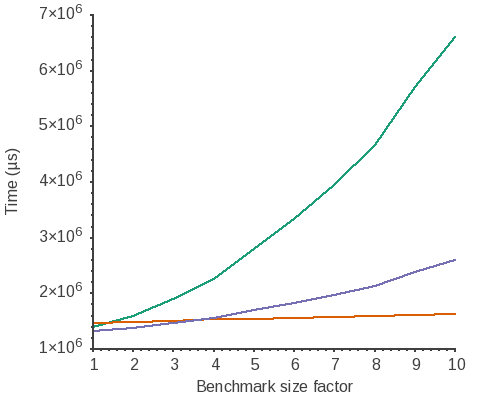
\includegraphics[scale=0.5]{images/bf-consecutive_loops.png}
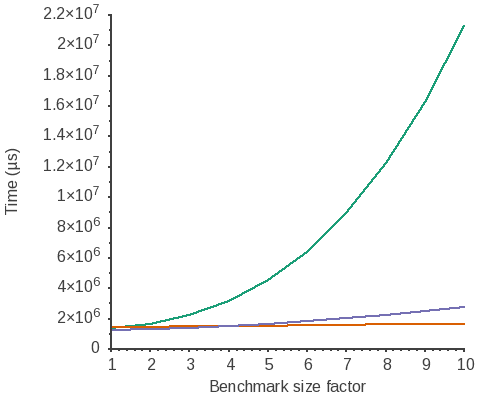
\includegraphics[scale=0.5]{images/bf-imbricated_loops.png}
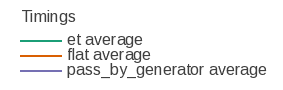
\includegraphics[scale=0.5]{images/bf-graph-legend.png}
\caption{
  Compiler execution time measurements for consecutive loops (left)
  and nested loops (right)
}\label{fig:bf-bench}
\end{figure}

Figure \ref{fig:bf-bench}
both highlight considerably higher compiler execution times for the expression
template based backend, high enough to suggest that the use of expression
templates induces an overhead higher than parsing and generating Brainfuck
programs using the pass-by-generator backend. However the pass-by-generator
backend still has a compile time overhead much higher than the flat backend,
which shows near constant compiler execution times on these small scale
benchmarks.

Finally, AST deepening has a much higher impact on compile times than AST
widening with the expression template backends, whereas the other backends seem
to scale similarly as the AST grows wider or deeper.

\subsubsection{
  Large Brainfuck programs
}

The following benchmarks consist in measuring compiler execution times for
compiling Brainfuck code examples. These example programs are also used to
validate the metacompiler's backend implementations by compiling them and
verifying their output.

\begin{itemize}
\item A Hello World program (106 tokens).
\item The same Hello World program, ran twice (212 tokens).
\item A Mandelbrot set fractal viewer (11672 tokens).
\end{itemize}

\begin{figure}
\begin{tabular}{|c|c|c|c|}
\hline
Backend             & Hello World & Hello World x2  & Mandelbrot \\
\hline
Flat                & 1.81        & 2.25            & 49.68 \\
Pass-by-generator   & 9.77        & 34.37           & Failure (timeout) \\
Expression template & 50.60       & 192.73          & Failure (timeout) \\
\hline
\end{tabular}
\caption{BF compile time measurements in seconds
}\label{fig:BF-compile-times}
\end{figure}

The measurements in figure \ref{fig:BF-compile-times} help us better understand
how various metacompiling techniques behave at scale. The "Flat" backend shows
very good performance on all examples, including the Mandelbrot example that is
about 100 times larger than the Hello World example. However the other cases
highlight severe scaling issues and tend to confirm our previous hypothesis
being that using generator functions to pass values makes the code generation
quadratic. Finally, the "Expression template" backend performance highlights
heavy performance impact when expression templates are being used, which is
likely due to the complexity of the mechanisms expression templates involve like
SFINAE and overload resolution.

\subsubsection{
  Conclusions
}

\end{document}
